\subsection{Metodologia}
\label{cha:subsecmetodologia}

Será definido um estudo comparativo para avaliação de performance entre SGBDs de código fechado: Oracle, SQL Server e CACHE. A implementação será feita utilizando a linguagem C{\#} .NET.

\subsection{Definição do esquema de dados}
\label{cha:sub1esquema}


\begin{figure}[ht!]
	\begin{center}
		%%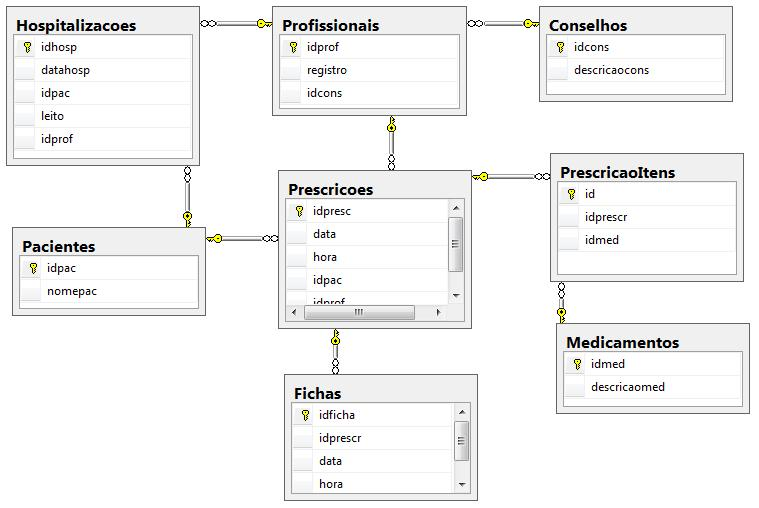
\includegraphics[width=10in,height=6in]{esquema.jpg}
		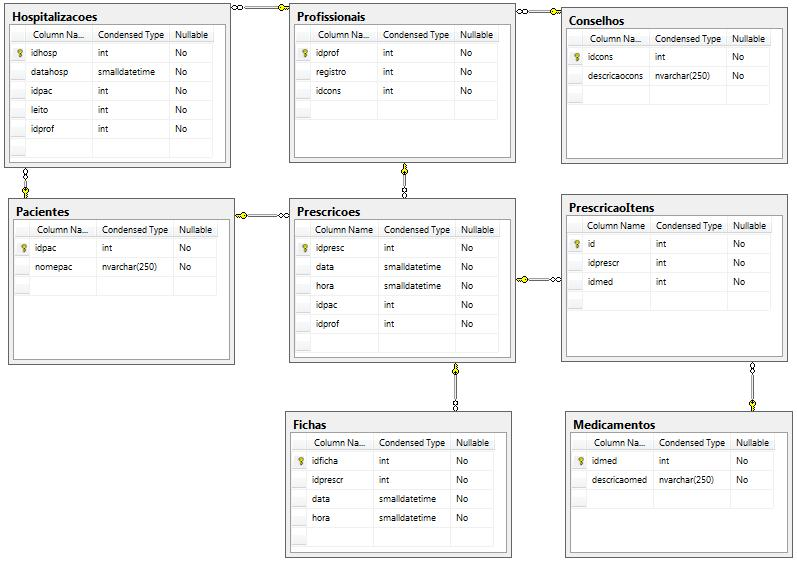
\includegraphics[scale=0.7]{esquema2.jpg}
		\caption{\label{esquema} Base de dados para execução dos testes}		
	\end{center}
\end{figure}


O esquema de dados é o conjunto de descrições que definem os tipos de dados e sua organização para o sistema de gerenciamento de banco de dados. Podem existir muitos tipos diferentes de dados, dependendo da complexidade do banco de dados.
Mesmo os sistemas de banco de dados mais simples diferenciam dados numéricos e de texto. Em bancos de dados mais
complexos, o esquema diferencia níveis de dados numéricos, além de identificar outras características dos dados.

Ao migrar o banco de dados, o esquema pode ser um desafio importante. É necessário mapear os tipos de dados do banco
de dados antigo para os tipos de dados do novo sistema de banco de dados. Eles não precisam ter o mesmo nome, mas
devem ter a mesma função. Por exemplo, se voce não mapear os tipos de dados corretamente na migração do banco de dados, podem ocorrer resultados imprevisíveis nas buscas, pior ainda, dados podem ser danificados ou perdidos.

O esquema também pode indicar relações entre tabelas. Estas relações definem a integridade referencial. Integridade referencial é uma das áreas problemáticas em gerenciamento de banco de dados, principamente se os usuarios que acessam os dados não conhecem as definições de referencias e não respeitam tais regras, para isso um bom sistema gerenciador de banco de dados deve implementar um bom mecanismo de verificação de integridade referencial.

Quanto a integridado de dados, um problema encontrado em varios bancos de dados antigos é a falta de tipagem nos dados armazenados, tornando a migração mais lenta pois é necessário a verificação dos tipos de dados nas tabelas do banco novo.

Para avaliação de performace será criado um esquema de dados de média complexidade para avaliar os aspectos necessários em um bom 
sistema de banco de dados, a figura \ref{esquema} ilustra o esquema de dados.

\subsection{Esquema de Execução do estudo comparativo}
\label{cha:sub2esquema}

Serão definidas oito tabelas relacionadas e com campos de tipos diferentes para avaliar os diferentes requisitos referêntes a intergridade dos dados e referêntes a ralacionamentos entre as tabelas.

O esquema de execução de testes consiste em estabelecer conexão com o banco de dados, marcar tempo de inicio, executar as inserções ou consultas, liberar conexão, e marcar tempo final. Nesse tempo serão executados e avaliados os seguintes testes:

- Teste de integridade de dados: 

O teste deve verificar o quanto o SGDB  controla automaticamente a integridade dos diversos tipos de dados necessários ao modelo de dados definido. O teste constitui em definir os tipos de dados de cada atributo de cada tabela e verificar a garantia de integridade dos dados;

- Teste de integridade referencial:

O teste deve verificar o nível de controle de integridade em relação a inclusão, alteração e remoção de dados de tabelas que estão relacionadas com outras tabelas.

- Teste de integridade de chave primaria:

O teste deve verificar a integridade com relação a unicidade de chaves primarias nas tabelas.

- Teste de consistência de dados:

O teste deve verificar o controle que o SGBD tem sobre os tipos de dados que fornece. O presente teste é decorrência do primeiro visto que a garantia de integridade dos dados afeta profundamente a garantia de consistência.

- Teste de performance com utilização de tabelas comuns solitárias:

O teste deve verificar se o tempo de armazenamento e recuperação de informações utilizando somente dados do tipo texto e ou numéricos em tabelas sem relacionamento é satisfatório.

- Teste de performance com utilização de tabelas com relacionamentos:

O teste deve verificar o tempo de armazenamento e recuperação de informações utilizando somente dados do tipo texto e ou numéricos em tabelas um ou mais relacionamentos.

- Teste de acesso concorrente:

O teste deve verificar a performance do sistema variando a quantidade de usuários acessando simultâneamente os dados.

A Execução dos testes será realizada remotamente e localmente, com o objetivo de avaliar tambem influências de uma rede no estabelecimento da conexão.

\subsection{Bancos de dados}
\label{cha:conhecendo}

\subsubsection{SQL Server} 

O SQL Server é um SGBD (sistema gerenciador de Banco de dados) relacional criado pela Microsof. É um Banco de dados robusto e usado por sistemas corporativos dos mais diversos portes.

É um banco de dados projetado para ser executado em plataformas que vão de laptops a servidores multiprocessador de grande porte. SQL Server é comumente usado como o sistema de infra-estrutura para sites e CRMs das empresas e pode suportar milhares de usuários simultâneos.

SQL Server vem com uma série de ferramentas para ajudá-lo com o seu banco de dados e administração de tarefas de programação.

SQL Server é muito mais robusta e escalável que um sistema de gestão de dados desktop como o Microsoft Access. Quem já tentou usar o Access como um back-end para um site provavelmente deve estar familiarizado com os erros que foram gerados quando muitos usuários tentaram acessar o banco de dados!

Embora o SQL Server também pode ser executado como um sistema de banco de dados desktop, é mais comumente usado como um sistema de banco de dados do servidor. \cite{sqlserver}

\subsubsection{Oracle}

O Oracle é um SGBD que surgiu no fim dos anos 70. O SGBD da Oracle é líder de mercado. O Oracle 9i foi pioneiro no suporte ao modelo web. O Oracle 10g, mais recente, se baseia na tecnologia de grid. Recentemente fora lançado o Oracle 11g que veio com melhorias em relação ao Oracle 10g.

Além da base de dados, a Oracle desenvolve uma suíte de desenvolvimento chamada de Oracle Developer Suite, utilizada na construção de programas de computador que interagem com a sua base de dados.

A Oracle também criou a linguagem de programação PL/SQL, utilizada no processamento de transações. \cite{oracle}

\subsubsection{Caché} 

Caché é um sistema de gerenciamento de banco de dados proprietário, produzido pela InterSystems, baseado na Tecnologia M.
A empresa descreve o banco como pós-relacional, e afirma que: oferece uma visão relacional e orientada a objetos dos mesmos dados, sem necessidade de mapeamentos ou redundância.

A arquitetura unificada do Caché suporta aplicativos orientados a objeto e relacionais utilizando SQL ANSI.

O Caché permite rápido desenvolvimento de aplicações Web, processamento transacional de alta performance, escalabilidade maciça, e consultas em tempo real de dados transacionais, além de baixíssimas necessidades de manutenção

Caché suporta diversas linguagem de programação, entre elas ObjectScript, um superconjunto funcional da linguagem M (Padrão ANSI para a linguagem MUMPS). Por motivos de mercado, a empresa prefere manter o produto Caché afastado desse nome. Os principais clientes de Caché são hospitais e financeiras americanos.

Na prática, Caché é a evolução a longo prazo da tecnologia M. Seu desempenho é considerado por muitos superior ao de SGDBRs tradicionais.

A visão pós-relacional de Caché também pode ser vista como uma visão pré-relacional e atualmente seria melhor descrita como uma visão não-relacional já que internamente Caché guarda seus dados em matrizes multi-dimensionais capazes de carregar dados estruturados hierarquicamente. Curiosamente, a tecnologia adequada para modelo de dados hierárquico sobreviveu e a total dominação do modelo relacional no mercado e hoje apresenta uma estrutura que pode ser, pelo menos em algumas aplicações, mais adequada para guardar objetos ou dados em XML.

O caché suporta modelagem de dados relacional ou orientado a objetos. \cite{cache}

\subsection{Testes com conexao com o Banco}
\label{cha:conexao}

\subsubsection{SQL Server}

Existem inúmeras formas de estrabelecer conexao com o banco, tudo depende da aplicação, existem maneiras standard de conexão que não fornecem muita segurança e existem mecanismos mais sofisticados de estabelecer conexão de maneira muito segura, abaixo alguns exemplos:

\scriptsize

\begin{verbatim}

Standard Security:

Data Source=myServerAddress;Initial Catalog=myDataBase;User Id=myUsername;Password=myPassword;

Standard Security alternative syntax

Server=myServerAddress;Database=myDataBase;User ID=myUsername;Password=myPassword;Trusted_Connection=False;

Trusted Connection:

Data Source=myServerAddress;Initial Catalog=myDataBase;Integrated Security=SSPI;

Trusted Connection alternative syntax

Server=myServerAddress;Database=myDataBase;Trusted_Connection=True;

\end{verbatim}

\normalsize

Será avaliada a string de conexão que estabelece conexão com o banco no menor tempo possível. \cite{sqlstring}

\subsubsection{Oracle}

Existem variadas formas de se estabelecer conexão com um Banco Oracle, assim como o SQL Server, utilizando objetos que recebem uma string de conexão, assim sendo tambem será testada que tipo de conexão é mais rapida. Abaixo seguem alguns exemplos.

\scriptsize

\begin{verbatim}

Using TNS
Data Source=TORCL;User Id=myUsername;Password=myPassword;

Using integrated security
Data Source=TORCL;Integrated Security=SSPI;

Using ODP.NET without tnsnames.ora
Data Source=(DESCRIPTION=(ADDRESS_LIST=(ADDRESS=(PROTOCOL=TCP)(HOST=MyHost)(PORT=MyPort)))
(CONNECT_DATA=(SERVER=DEDICATED)(SERVICE_NAME=MyOracleSID)))
;User Id=myUsername;Password=myPassword;

\end{verbatim}

\normalsize

Será avaliada a string de conexão que estabelece conexão com o banco no menor tempo possível. \cite{orastring}

\subsubsection{Caché}

\scriptsize
\begin{verbatim}

Standard
DRIVER={InterSystems ODBC};SERVER=myServerAddress;DATABASE=myDataBase;UID=myUsername;
PWD=myPassword;

Specifying port
DRIVER={InterSystems ODBC};SERVER=myServerAddress;PORT=12345;DATABASE=myDataBase; UID=myUsername;
PWD=myPassword;
 
Specifying protocol
DRIVER={InterSystems ODBC};SERVER=myServerAddress;PORT=12345;DATABASE=myDataBase;PROTOCOL=TCP;
STATIC CURSORS=1;UID=myUsername;PWD=myPassword;

\end{verbatim}

\normalsize

Será avaliada a string de conexão que estabelece conexão com o banco no menor tempo possível. \cite{cacstring}



\subsection{Testes de integridade de dados ou de domínio}
\label{cha:integridade}


Quando falamos em integridade, pensamos em proteção contra hackers e ataques do gênero, ou até mesmo backup, mas a integridade começa em um nível muito mais baixo que isto, começa na criação e projeto do banco de dados.

Integridade de domínio nada mais é do que a integridade do campo como o tipo de dados correto, se permite null ou not null, defaults, checks constraints, estes mecanismos foram criados para dar integridade aos campos. Os tipos de dados também são caracterizados como integridade de domínio, se o tipo de dado estiver incorreto, ou com mais posições que o necessário, pode haver ali um risco que quebre a integridade. O check aqui é em nível de campo apenas por exemplo: Tenho um campo Meses e quero que entre valores de 1 até 12 somente.

No estudo que será realizado testes quanto aos tipos de dados criados nas tabelas, serão executadas tentativas de inserir dados não compatíveis com os dados definidos nas tabelas, será avaliado que tipo de resposta o banco retorna e o tempo de resposta do banco de dados quando existir tentativas de inserção de dados de domínios diferentes.

\subsection{Testes de integridade referencial}
\label{cha:intref}

A integridade referencial é mais conhecida, são as \emph{Foreign Keys}, nada mais é que eu aceitar valores em minha entidade que estão em outra entidade, isto é possível a partir da integridade de entidade, eu apenas consigo criar \emph{Foreign Keys} a partir de uma \emph{Primary Key} ou uma \emph{Unique}, a integridade referencial consiste também em check em nível de tabela e não em nível de campo, no ato da criação da tabela crio um check, por exemplo:

Tenho uma tabela com 2 campos Medico1, Medico2, e quero que um dos campos sempre seja preenchido não importa qual, para isto preciso de um check em nível de tabela.

Segue tabela de tipos de integridade :

\begin{center}
	\begin{tabular}{ll}
		Tipos de Integridade & Tipo de constraint \\
		Dominio & DEFAULT, CHECK, REFERENCIAL \\
		Entidade & PRIMARY KEY, UNIQUE \\
		Referencial & FOREIGN KEY, CHECK \\
	\end{tabular}
	\captionof{table}{Tipos de integridade e constraints}
	\label{tab:intref}
\end{center}


Para se adicionar integridade a uma tabela é possível fazê-lo de duas maneiras CREATE TABLE ou ALTER TABLE.

É possível aplicar integridade de duas maneiras : Declarativa e Procedural

Declarativa: É declarado como parte da definição do objeto, e o SQL automaticamente assume o critério, é o método preferido pela maioria, para se determinar esta integridade basta usar os checks constraints, defaults e os rules.

Procedural: É definido com o script do objeto, é utilizado mais para lógicas muito complexas e exceções, um bom exemplo de integridade procedural é um delete em cascata, a integridade procedural pode ser realizada no cliente ou no servidor, é conseguida através de stored procedures e triggers.



\begin{center}
	\begin{tabular}{llll}

	Integridade & Funcionalidade & Custo em performance & Modificação Antes/Depois \\
	Constraints & Médio & Baixo & Antes \\
	Defaults e Roles & Baixo & Baixo & Antes \\
	Triggers & Alto & Médio-Alto & Depois \\
	Tipo de dados & Baixo & Baixo & Antes \\
	Null, Not Null & Baixo & Baixo & Antes \\


	\end{tabular}
	\captionof{table}{Tipos de constraints e custos em performance}
	\label{tab:intref2}
\end{center}

Obs : As rules estão na versão do SQL 2000 por exemplo, por compatibilidade, não são recomendados, a constraint Default, veio para substituí-la porque exige menos recurso para ser executada.

A integridade dos dados é algo muito importante e existem recursos para certificar isto, porém existem meios melhores que outros de se prover de integridade em meio aos recursos, é totalmente errado transferir esta funcionalidade para a aplicação, por exemplo, criar uma procedure ou function na aplicação para checar se já existe algum valor antes de inserir, porque a tabela não possui chave primária, aplicações são sempre refeitas ou alguma nova é criada que utilize um mesmo banco de dados, por isto estas regras pertinentes a dados devem permanecer na base de dados e não na aplicação.

E uma tabela sem chave primária está sem integridade de entidade, e pode sofrer falhas pertinentes a este tipo de falta de integridade, falhas esta que podem ser vistas somente depois de muito tempo que o banco está em funcionamento, causando um enorme transtorno para corrigir lacunas que estão vazias e não poderiam, valores duplicados e não poderiam, valores inválidos inseridos. Isto sim dá trabalho de se corrigir.

Sempre os recursos de integridade que tem baixo custo de performance (tabela \ref{tab:intref2}), e sua modificação ocorrem antes do valor ser inserido são as melhores para se aplicar ao banco, porque exigem pouco do banco e são rápidos. Você pode perguntar, então nunca usarei triggers? As triggers porém tem seu espaço, triggers são um tipo de stored procedures que são bastante utilizadas em lógicas muito complexas, que as constraints não cobrem como: Emitir mensagens customizadas, verificar valores em outras tabelas no ato do update/insert, executar antes das constraints (instead off) e execução em cascata.

No estudo que será realizado será feito testes para verificar se, existindo relacionamento entre tabelas, o banco verifica e bloqueia tentativas de exclusão de dados relacionados e será avaliado o tempo de resposta do banco quando na tentativa de violar relacionamentos definidos na criação das bases de dados.

\subsection{Testes de integridade de chave primaria}
\label{cha:intchave}

A integridade de chave primária nada mais é que a integridade da tabela, isto é conseguido através das \emph{Primary Keys} ou \emph{Uniques}, uma tabela sem PK ou Unique é uma tabela sem integridade de entidade, é muito comum pegarmos tabelas sem PK, alguns colocam campo identity e não se preocupam com as PKs, mas esquecem que o campo identity não garante a não duplicidade.

No estudo que será realizado nos campos identificados como chave primária, será executado testes quanto a inserção de valores duplicados em campos definidos como chave primária e UNIQUE, será avaliado o tipo de retorno e o tempo de resposta.

Será avaliado a capacidade do banco de gerenciar os campos definidos como chave primaria, e o tempo de resposta quando existir tentativa de quebra de integride.

\subsection{Testes de consistência de dados}
\label{cha:concistencia}

Falar de consistencia de dados é falar de estado do banco antes e após transações, se o banco deve manter consistencia de dados após qualquer tipo de transação.

A consistencia do banco influi fortemente nos quesitos anteriores de validação, pois se ouver modificação em tabelas relacionadas em uma transação, a coerencia dos dados do banco deve ser mantida caso ocorra alguma falha no fluxo da transação, existindo o bom funcionamento dos mecanismos de RollBack.

Neste aspecto será avaliado tal mecanismo de manutenção da consistencia dos dados no banco. 

\subsection{Testes de performance com utilização de tabelas comuns solitárias}
\label{cha:perfsimples}

Os testes que serão feitos quanto a este quesito apenas verificarão a velocidade de inserção, update e delete em tabelas sem qualquer relacionamento, será avaliado o tempo de execução ao final das transações.


\subsection{Testes de performance com utilização de tabelas com relacionamentos}
\label{cha:perfrela}


Os testes realizados neste quesito, tem como objetivo avaliar o tempo que o banco leva para verificar inserções, updates e deletes em tabelas que possuem relacionamentos complexos, ou seja, entre mais de 2 tabelas. Transações serão disparadas para avaliar a validação de procedimentos mais robustos que vão requerer avaliação de que tipo de estrutura melhor se adapta em termos de performace em uma estrutura de dados complexa


\subsection{Testes de acesso concorrente}
\label{cha:con correncia}


Para avaliar acesso concorrente será criada uma aplicação que simule varias threads concorrendo por acesso ao banco, conexão, inserts em mesmas tabelas, updates e deletes.

Os tempos totais serão armazenados e avaliados ao final das execuções.





